\documentclass{article}

\usepackage{graphicx}
\usepackage{tikz}
\usepackage{tikzsymbols}
\usetikzlibrary{calc,patterns,shapes.geometric}
\pagestyle{empty}
\usepackage[margin=0pt]{geometry}
\geometry{papersize={14in,12in}}

\def\centerarc[#1](#2)(#3:#4:#5){\draw[#1] ($(#2)+({#5*cos(#3)},{#5*sin(#3)})$) arc (#3:#4:#5);}

\begin{document}
	\begin{figure}
		\centering
		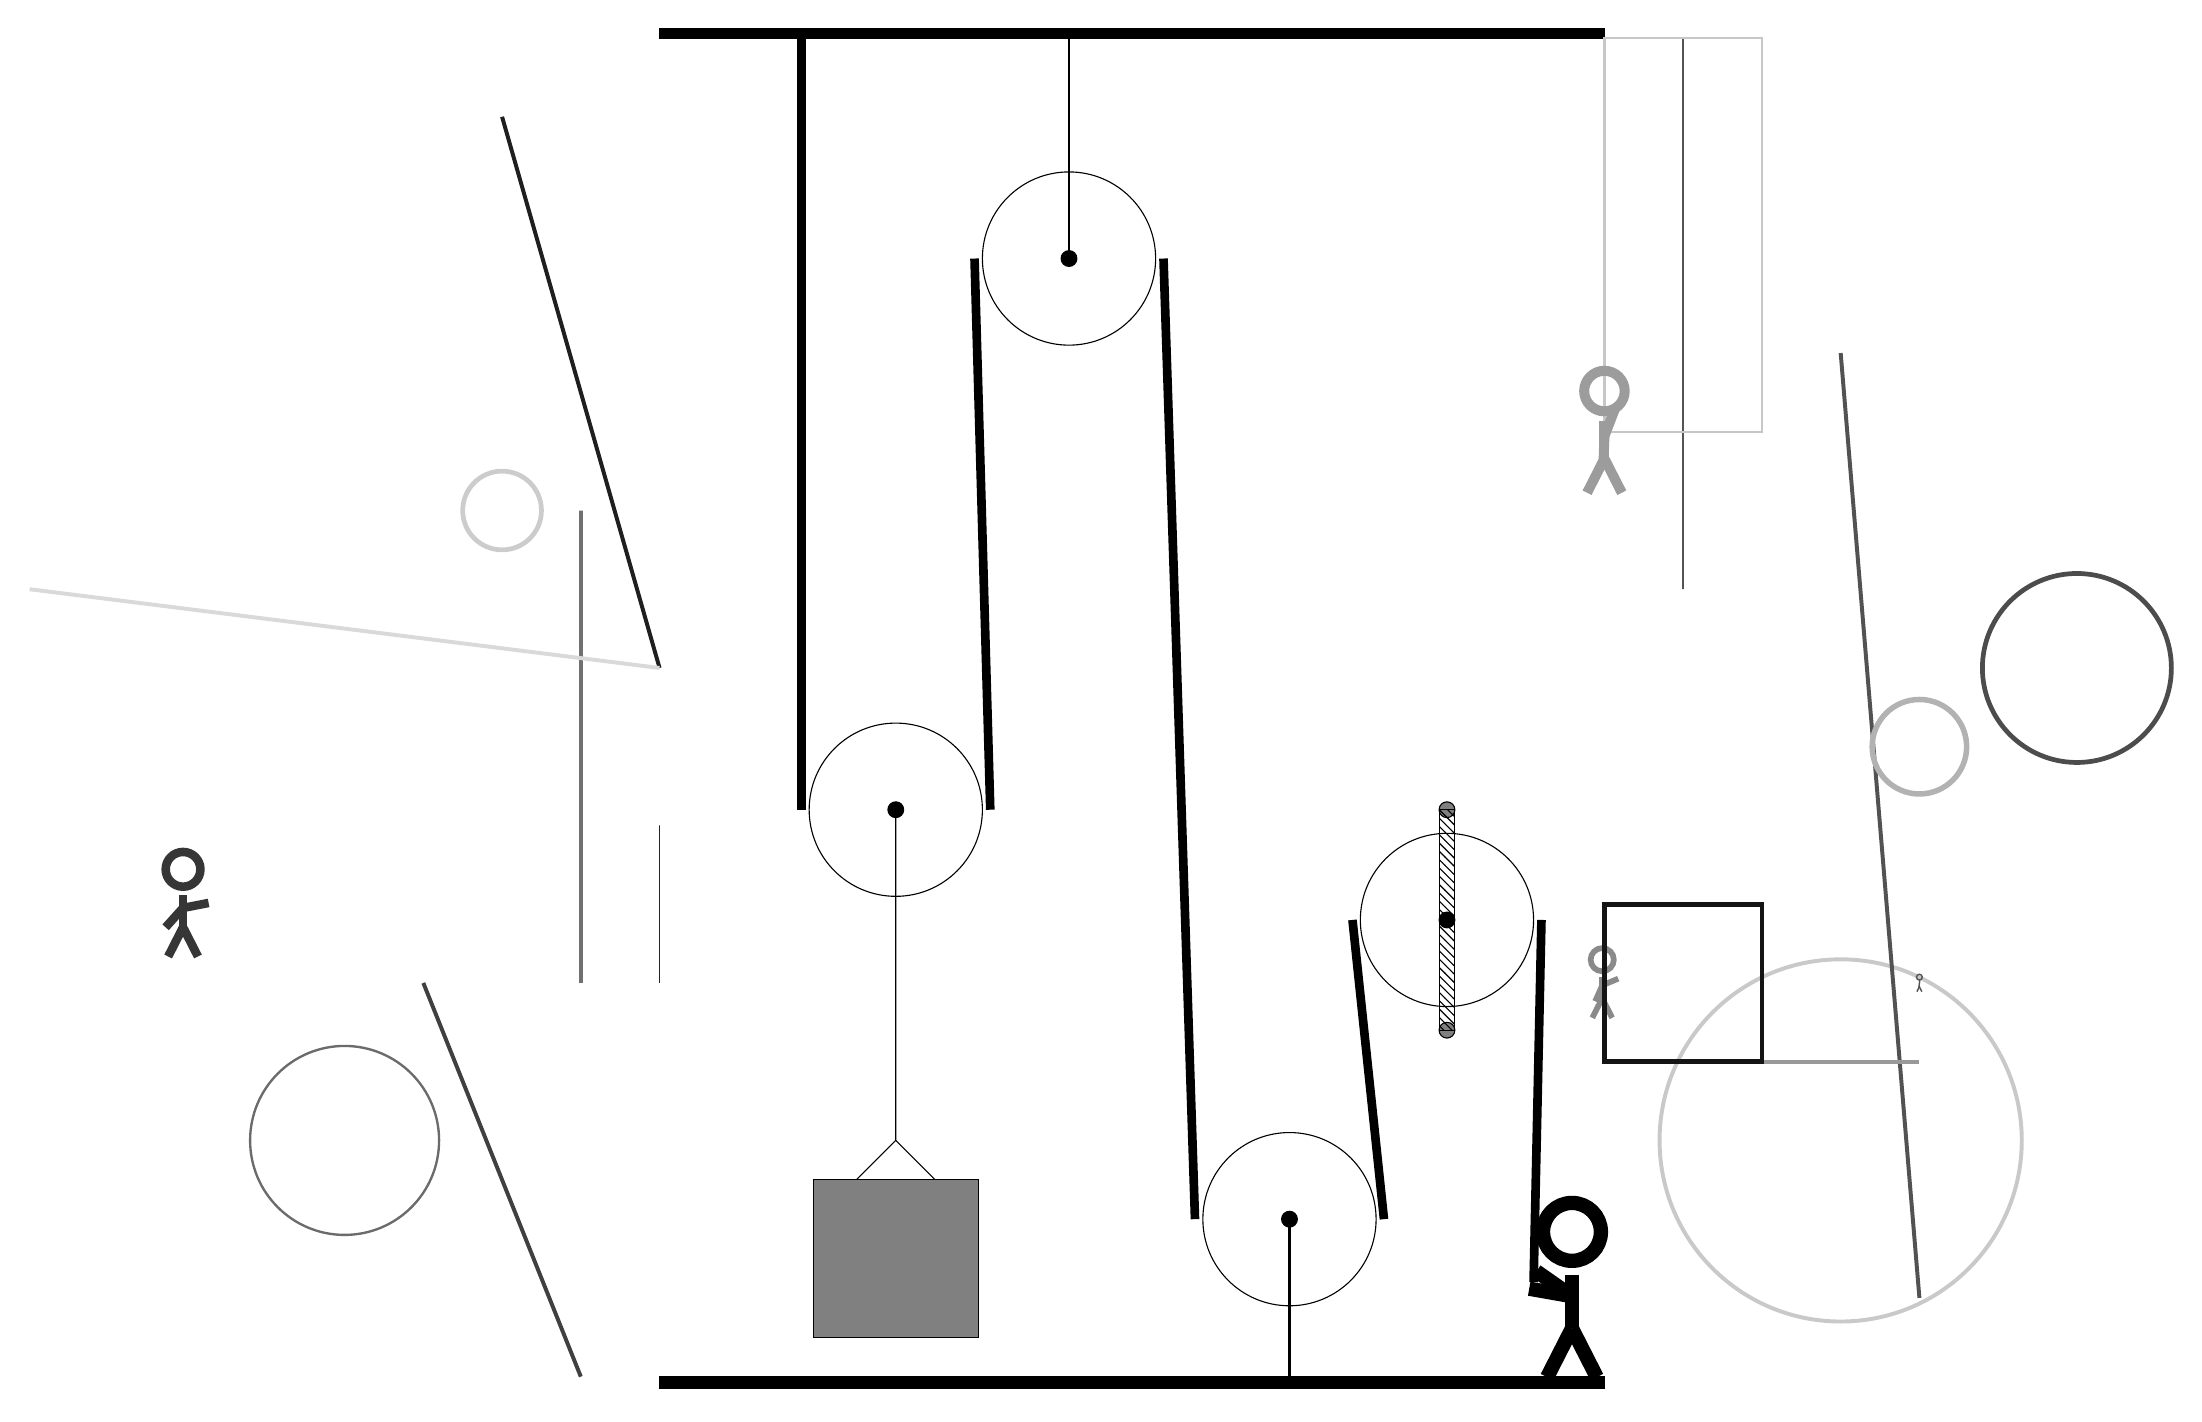
\begin{tikzpicture}
			%%%%% START %%%%%
			
			\draw[fill=black] (-2, 14) rectangle (10, 14.125);
			
			\draw (1, 4.2) circle (1.1);
			\draw[fill=black] (1, 4.2) circle (0.1);
			
			\draw (3.2, 11.2) circle (1.1);
			\draw[fill=black] (3.2, 11.2) circle (0.1);
			\draw[thick] (3.2, 11.2) -- (3.2, 14);
			
			\draw [line width=0.5mm, color=black!21](13, 0) circle (2.3);
			
			\draw[line width=0.5mm, color=black!68](13, 10) -- (14, -2);
			\draw [line width=0.6mm, color=black!70](16, 6) circle (1.2);
			\draw[line width=0.5mm, color=black!88](-2, 6) -- (-4, 13);
			
			\draw[line width=0.5mm, color=black!56] (-3, 8) rectangle (-3, 2);
			\draw[line width=0.5mm, color=black!75](-3, -3) -- (-5, 2);
			
			\draw[line width=0.5mm, color=black!40](14, 1) -- (10, 1);
			\node[line width=0.2mm, color=black!79] at (-8, 3) {\Strichmaxerl[6][48][11]};
			\node[line width=0.7mm, color=black!46] at (10, 2) {\Strichmaxerl[4][66][23]};
			\draw [line width=0.3mm, color=black!58](-6, 0) circle (1.2);
			\draw [line width=0.6mm, color=black!20](-4, 8) circle (0.5);
			
			\draw[line width=0.3mm, color=black!67] (11, 14) rectangle (11, 7);
			\node[line width=0.7mm, color=black!67] at (14, 2) {\Strichmaxerl[1][82][84]};
			
			\draw[line width=0.5mm, color=black!15](-2, 6) -- (-10, 7);
			\draw[line width=0.2mm, color=black!86] (-2, 2) rectangle (-2, 4);
			\draw [line width=0.7mm, color=black!30](14, 5) circle (0.6);
			\draw[line width=0.3mm, color=black!22] (12, 14) rectangle (10, 9);
			\draw[line width=0.6mm, color=black!92] (10, 3) rectangle (12, 1);
			\node[line width=0.6mm, color=black!39] at (10, 9) {\Strichmaxerl[7][88][69]};
			
			\draw (6, -1) circle (1.1);
			\draw[fill=black] (6, -1) circle (0.1);
			\draw[thick] (6, -1) -- (6, -3);
			
			\draw[fill=white](8, 2.8) circle (1.1);
			\draw[fill=black] (8, 2.8) circle (0.1);
			\draw[fill=black!50] (8, 4.2) circle (0.1);
			\draw[fill=black!50] (8, 1.4) circle (0.1);
			\draw[pattern=north west lines, pattern color=black] (7.9, 4.2) rectangle (8.1, 1.4);
			
			\draw (1, 4.2) -- (1, 0) -- (0.5, -0.5);
			\draw (1, 0) -- (1.5, -0.5);
			\draw[fill=black!50] (-0.05, -0.5) rectangle (2.05, -2.5);
			
			\draw[line width=1.1mm] (-0.2, 14) -- (-0.2, 4.2);
			\centerarc[line width=1.1mm](1, 4.2)(180:360:1.2000000000000002);
			\draw[line width=1.1mm](2.2, 4.2) -- (2.0, 11.2);
			\centerarc[line width=1.1mm](3.2, 11.2)(0:180:1.2000000000000002);
			\draw[line width=1.1mm](4.4, 11.2) -- (4.8, -1);
			\centerarc[line width=1.1mm](6, -1)(180:360:1.2000000000000002);
			\draw[line width=1.1mm](7.2, -1) -- (6.8, 2.8);
			\centerarc[line width=1.1mm](8, 2.8)(0:180:1.2000000000000002);
			\draw[line width=1.1mm](9.2, 2.8) -- (9.1, -1.8);
			
			\node at (9.5, -1.9) {\Strichmaxerl[10][-35][170]};
			
			\draw[fill=black] (-2, -3) rectangle (10, -3.15);
			
			%%%%% END %%%%%
		\end{tikzpicture}
	\end{figure}	
\end{document}